\documentclass[11pt]{article}
\usepackage[utf8]{inputenc}
\usepackage{amsmath}
\usepackage{amssymb}
\usepackage{amsthm}
\usepackage{tcolorbox}
\usepackage{tikz}
\usetikzlibrary{positioning}
\usepackage{graphicx}
\usepackage{natbib}
\usepackage{bibentry}
\usepackage[nottoc]{tocbibind}

\usepackage{mathtools}
\mathtoolsset{showonlyrefs}
\bibliographystyle{plainnat}
\numberwithin{equation}{section}

\newcommand{\argmax}[1]{\underset{#1}{\operatorname{arg}\,\operatorname{max}}\;}
\newcommand{\expectation}[1]{\mathbb{E}\left[#1\right]}
\newcommand{\Tr}[1]{\text{Tr}\left(#1\right)}
\newcommand{\x}{{\bf x}}
\newcommand{\z}{{\bf z}}
\newcommand{\N}{\mathcal{N}}

\newtheorem{proposition}{Proposition}[section]
\newtheorem{theorem}{Theorem}[section]

\title{Kalman Filters: an introduction}
\author{Gerardo Durán Martín}
\begin{document}
% Add everything to bibliography, even if it is not cited.
\nocite{*}

\maketitle

\section{Introduction}

Dynamical systems are models that capture the time evolution of a system \cite{strogatz}. A discrete-time linear dynamical system is a dynamical system in which an $M$-dimensional vector $\x_n$ evolves in the form.

\begin{equation}
	\x_{n+1} = {\bf A x}_n.
\end{equation}

% An example of a linear dynamical system is...
\begin{figure}[h!]
	\centering
	\includegraphics[scale=0.5]{../figures/discrete-dynamical-system}
	\caption{Example of a discrete-time dynamical system.}
	\label{fig:discrete-dynamical-system}
\end{figure}



In this work, we are interested in dynamical systems that depend on some unobserved signal, usually called latent variables, and a set of observed values that are directly derived from the source signal. We define the set of observed variables ${\bf X} = \{\x_n \in \mathbb{R}^M \vert n=1,\ldots, N\}$ as the observed dataset, and the set of latent variables ${\bf Z} = \{\z_n \in \mathbb{R}^K \vert n=1,\ldots, N\}$ as the latent dataset. We also denote $\mathcal{D} = ({\bf X}, {\bf Z})$ as the complete-dataset.

One way to represent such system is to assume the existence of an unobserved signal $\z_n$ that evolves linearly over time according to the matrix ${\bf A}\in\mathbb{R}^{K\times K}$. Once $\z_{n+1}$ is obtained, the observed value $\x_{n+1}$ is the result of a linear transformation over $\z_{n+1}$ induced by the matrix ${\bf C}\in \mathbb{R}^{M\times K}$. The equations that govern such system can be written as follows:

\begin{align*}
	\z_{n+1} &= {\bf A} \z_{n},\\
	\x_{n+1} &= {\bf C} \z_{n+1}.
\end{align*}

An example of such system is presented in Figure \ref{fig:hidden-dynamical-system}, in which the dynamics of the vector $\x_n$ is completely determined by the vector $\z_n$. Hence, the evolution of the system is completely determined by the initial condition $\z_0$. Assuming that $\z_0$ is known and we observed a fixed number of $N$ observations, the problem reduces to find matrices ${\bf A}$ and ${\bf C}$ that generated the observed values.

% An example of a linear dynamical system is...
\begin{figure}[h!]
	\centering
	\includegraphics[scale=0.5]{../figures/hidden-dynamical-system}
	\caption{Example of a hidden dynamical system. The blue arrows represent the underlying (hidden) system, whereas the orange arrows represent the observed system.}
	\label{fig:hidden-dynamical-system}
\end{figure}

In some settings, however, we assume that the underlying signal $\z_n$ and the observed value $\x_n$ do not behave deterministically. For example, suppose we are interested in modelling the behaviour of a stock. We assume that the stock has an underlying signal that is then affected by stochastic market forces and corrupts its underlying value. Under this scenario, ${\bf X}$ is a dataset of sampled random values that were generated by some unseen dataset ${\bf Z}$. Our goal in this work is to find a probabilistic model that efficiently estimates the parameters of our model, and a procedure to determine the plausible dataset $\bf Z$.

% * double check writing;
% * add reference to observed (X) and latent (Z) dataset
In this work, we show that if the proposed model is linear with Gaussian noise, we can make use of the EM algorithm to obtain the model parameters, and estimate the underlying latent dataset using a procedure known as Kalman Filtering.

\subsection{Linear dynamical systems with added noise}
We begin this section by modifying our previous system by adding uncertainty into the system. We follow from the ideas presented in \cite{prml}. As previously mentioned, we assume that that both the underlying signal and the observed signal are corrupted by some noise. That is

\begin{align*}
	\z_{n+1} &= {\bf A} \z_{n} + \boldsymbol\varepsilon_n,\\
	\x_{n+1} &= {\bf C} \z_{n+1} + \boldsymbol\varphi_n.
\end{align*}

The noise terms $\boldsymbol{\varepsilon}_n$, and $\boldsymbol{\varphi}_n$ are assumed to be normally distributed with mean zero and covariance matrices $\boldsymbol{\Gamma}$, and $\boldsymbol{\Sigma}$. An illustration of this modified system is presented in presented in figure \ref{fig:hidden-noisy-dynamical-system}.

\begin{figure}[h!]
	\centering
	\includegraphics[scale=0.5]{../figures/hidden-stochastic-dynamical-system}
	\caption{Example of a hidden dynamical system with added noise. The deterministic dynamics of the model are the same as the ones presented in figure \ref{fig:hidden-dynamical-system}. However, we consider }
	\label{fig:hidden-noisy-dynamical-system}
\end{figure}



Given the structure of the dynamical system, the likelihood of the model is given by

\begin{equation}
	p({\bf X}, {\bf Z} \vert\boldsymbol\theta) = p(\z_1)\prod_{n=2}^N p(\z_n\vert \z_{n-1})\prod_{n=1}^N p(\x_n\vert \z_n).
\end{equation}

% to-do: Add equations for the initial condition z0
We can also represent this system as a graphical model as specified in Figure \ref{fig:lds-gm}.

\begin{figure}
	\centering
	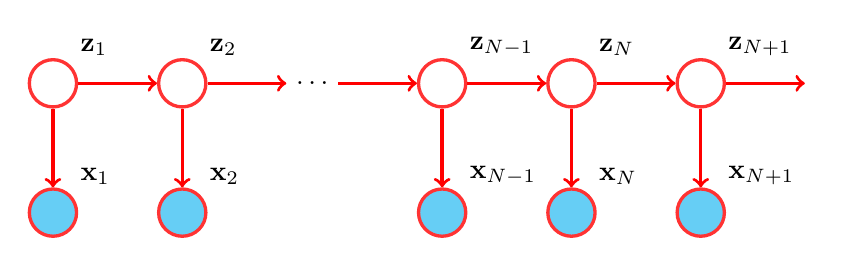
\begin{tikzpicture}[
latentnode/.style={circle, draw=red!80, minimum size=6mm, very thick},
observednode/.style={circle, draw=red!80, fill=cyan!60, minimum size=6mm, very thick},
]

% Defining the nodes
\node[latentnode, label=above right:{${\bf z}_1$}] (z1) {};
\node[latentnode, label=above right:{${\bf z}_2$}] (z2) [right=of z1] {};
\node (transition) [right=of z2] {$\ldots$};
\node[latentnode, label=above right:{${\bf z}_{N-1}$}] (z_nm1) [right=of transition] {};
\node[latentnode, label=above right:{${\bf z}_{N}$}] (zn) [right=of z_nm1] {};
\node[latentnode, label=above right:{${\bf z}_{N+1}$}] (z_np1) [right=of zn] {};
\node (final) [right=of z_np1] {};

% Defining observed nodes
\node[observednode, label=above right:{${\bf x}_1$}] (x1) [below=of z1]{};
\node[observednode, label=above right:{${\bf x}_2$}] (x2) [below=of z2]{};
\node[observednode, label=above right:{${\bf x}_{N-1}$}] (x_nm1) [below=of z_nm1]{};
\node[observednode, label=above right:{${\bf x}_{N}$}] (xn) [below=of zn]{};
\node[observednode, label=above right:{${\bf x}_{N+1}$}] (x_np1) [below=of z_np1]{};


% Relationships between latent variables
\draw[->, color=red, very thick] (z1) -- (z2);
\draw[->, color=red, very thick] (z2) -- (transition);
\draw[->, color=red, very thick] (transition) -- (z_nm1);
\draw[->, color=red, very thick] (z_nm1) -- (zn);
\draw[->, color=red, very thick] (zn) -- (z_np1);
% final node
\draw[->, color=red, very thick] (z_np1) -- (final);

% Relationships between observed and latent variables
\draw[->, color=red, very thick] (z1) -- (x1);
\draw[->, color=red, very thick] (z2) -- (x2);
\draw[->, color=red, very thick] (z_nm1) -- (x_nm1);
\draw[->, color=red, very thick] (zn) -- (xn);
\draw[->, color=red, very thick] (z_np1) -- (x_np1);

\end{tikzpicture}
	\caption{Graphical representation of a linear dynamical system with latent variables. The filled circles represent observed datapoints, whereas the empty circles represent latent variables.}
	\label{fig:lds-gm}
\end{figure}


% to-do: rewrite this paragraph. Motivate the EM algorithm by rewriting the log-likelihood and show that the resulting
% rewrite of equations lead to the E and the M steps. Furthermore, add that criterion for converge of the algorithm can be
% found on a paper (find paper)	
Our goal is to find the set of parameters $\boldsymbol\theta = \{{\bf A}, {\bf C}, \boldsymbol\Gamma, \boldsymbol\Sigma, \boldsymbol\mu_0, {\bf V}_0\}$ that best represent the data. From a frequentist perspective, this is done by maximising the likelihood of the data with respect to the parameters $\boldsymbol{\theta}$. Maximising the likelihood of this model, however, is not straightforward. This is because the only observed data we have is given by the observed dataset $\bf X$. % Explain more this step


\subsection{The EM algorithm}

% Reference to the EM algorithm?
One approach of finding such parameters is to make use of the EM algorithm: an iterative approach to maximise the likelihood of the complete-data log-likelihood as follows

\begin{align}
	\boldsymbol{\theta}^\text{new} &= \argmax{\boldsymbol{\theta}} \mathbb{E}_{\z\vert \x, \boldsymbol{\theta}^\text{old}}[\log p(\x, \z\vert \boldsymbol\theta)]\\
	&= \argmax{\boldsymbol{\theta}} Q(\boldsymbol\theta, \boldsymbol\theta^\text{old}).
\end{align}

Where we have defined $Q(\boldsymbol\theta, \boldsymbol\theta^\text{old}) := \mathbb{E}_{\z\vert \x, \boldsymbol{\theta}^\text{old}}[\log p(\x, \z\vert \boldsymbol\theta)]$. The computation of the posterior probability of latent variables $p(\z\vert \x, \boldsymbol\theta^\text{old})$ is called the E-step. The maximisation of the expected complete-data log-likelihood with respect to the posterior latent variables $Q(\boldsymbol\theta, \boldsymbol\theta^\text{old})$ is called the M-step.

We derive the EM algorithm considering the following three propositions.

\begin{proposition}
	The log-likelihood $\log p({\bf X} \vert \boldsymbol{\theta})$ can be written as the sum of two factors
	\begin{equation}
		\log p({\bf X} \vert \boldsymbol{\theta}) = \mathcal{L}(q, \boldsymbol{\theta}) + \text{KL}(q \vert\vert p).
	\end{equation}
	Where
	\begin{align}
		\mathcal{L}(q, \boldsymbol{\theta}) &= \int q({\bf Z})\log\left(\frac{p({\bf X}, {\bf Z} \vert \boldsymbol\theta)}{q({\bf Z})}\right) d{\bf Z},\\
		\text{KL}(q \vert\vert p) &= \int q({\bf Z}) \log\left(\frac{q({\bf Z})}{p({\bf Z}\vert {\bf X}, \boldsymbol\theta)}\right) d{\bf Z}.
	\end{align}
\end{proposition}

\begin{proof}
	\texttt{to-do: write proof}
\end{proof}

% to-do: it can be shown that the KL term is nonnegative (what are the conditions?). Set elements-information-theory as reference.


%to-do: define a set \mathcal Q of "valid" distributions.
\begin{proposition} (\textbf{E-step})
	The function $q$ that maximises the lower bound $\mathcal L(q, \boldsymbol{\theta}$) is given by
	\begin{equation}
		q = \max_{\hat q} \mathcal{L}(\hat q, \boldsymbol\theta) = p({\bf Z} \vert {\bf X}, \boldsymbol\theta).
	\end{equation}
\end{proposition}

\begin{proof}
	\texttt{to-do: write proof.}
\end{proof}

\begin{proposition}
	(\textbf{M-step}) Maximising $\mathcal{L}(q, \boldsymbol{\theta})$ over $\boldsymbol{\theta}$ at fixed $q({\bf Z}) = p({\bf Z} \vert {\bf X}, \boldsymbol\theta^\text{old})$ is equivalent to maximising the function
	\begin{equation}
		Q(\boldsymbol{\theta}, \boldsymbol{\theta}^\text{old}) = \mathbb{E}_{{\bf Z}\vert {\bf X}, \boldsymbol{\theta}^\text{old}}[\log p({\bf X}, {\bf Z}\vert \boldsymbol\theta)]
	\end{equation}
\end{proposition}

\begin{proof}
	\texttt{to-do: write proof.}
\end{proof}


\subsection{The E-step}
To make use of the E-step, it is helpful to distinguish which elements depend on $\z_n$. Consider

\begin{align}
	\log p({\bf X}, {\bf Z}\vert \boldsymbol\theta) &= \log p(\z_1) + \sum_{n=2}^N \log p(\z_n\vert \z_{n-1}) + \sum_{n=1}^N \log p(\x_n\vert \z_n)\\
	   &=\frac{1}{2}\log\vert{\bf V}_0^{-1}\vert - \frac{1}{2}(\z_1 - \boldsymbol\mu_0)^T{\bf V}_0^{-1}(\z_1 - \boldsymbol\mu_0) \nonumber \\
	   &\hspace{1cm}+ \sum_{n=2}^N \frac{1}{2}\log\vert\boldsymbol\Gamma^{-1}\vert - \frac{1}{2}(\z_n - {\bf A z}_{n-1})^T\boldsymbol{\Gamma}^{-1}(\z_n - {\bf A z}_{n-1}) \nonumber \\
	   &\hspace{1cm}+\sum_{n=1}^N \frac{1}{2}\log\vert\boldsymbol\Sigma\vert -\frac{1}{2}(\x_n - {\bf C z}_n)^T \boldsymbol{\Sigma}^{-1}(\x_n - {\bf C z}_n) + \text{const.}\\
	   &= \frac{1}{2}\log \vert
	  {\bf V}_0^{-1}\vert -\frac{1}{2}\left[\text{Tr}\left(\z_1 \z_1^T {\bf V}_0^{-1}\right) -2 \z_1^T{\bf V}_0^{-1}\boldsymbol\mu_0 + \boldsymbol\mu_0^T {\bf V}_0^{-1}\boldsymbol\mu_0\right] \nonumber \\
	  &\hspace{1cm}+ \frac{N-1}{2}\log\vert\boldsymbol\Gamma^{-1}\vert + \frac{N}{2}\log\vert \boldsymbol\Sigma^{-1}\vert \nonumber \\
	  &\hspace{1cm}-\frac{1}{2} \sum_{n=2}^{N}\text{Tr}\big(\z_n\z_n^T\boldsymbol\Gamma^{-1} -{\bf A} \z_{n-1}\z_n^T\boldsymbol\Gamma^{-1} - \nonumber\\
	  &\hspace{1.8cm}{\bf A}^T\boldsymbol{\Gamma}^{-1}\z_n\z_{n-1}^T + {\bf A}^T \boldsymbol\Gamma^{-1}{\bf A}\z_{n-1}\z_{n-1}^T\big) \nonumber\\
	  &\hspace{1cm}-\frac{1}{2}\sum_{n=1}^N\big[\x_n^T\boldsymbol{\Sigma}^{-1}\x_n - \z_n^T{\bf C}^T\boldsymbol\Sigma^{-1}\x_n - \x_n^T\boldsymbol{\Sigma}^{-1}{\bf C}\z_n  \\
	  &\hspace{1cm} + \text{Tr}(\z_n\z_n^T{\bf C}^T\boldsymbol\Sigma^{-1}{\bf C})\big] + \text{const.} \label{eq:complete-log-likelihood}
\end{align}

Where const. are the terms that do not depend on $\boldsymbol{\theta}$. From equation \eqref{eq:complete-log-likelihood}, we note that the expectation with respect to the posterior distribution comes only in the form of the expectations $\mathbb{E}[\z_n]$, $\mathbb{E}[\z_n\z_{n}^{T}]$, and  $\mathbb{E}[\z_n\z_{n-1}^{T}]$. That is,

\begin{align}
	Q(\boldsymbol\theta, \boldsymbol\theta^\text{old}) &= \frac{1}{2}\log \vert
	  {\bf V}_0^{-1}\vert -\frac{1}{2}\left[\text{Tr}\left(\mathbb{E}\left[\z_1 \z_1^T\right] {\bf V}_0^{-1}\right) -2 \mathbb{E}\left[\z_1\right]^T{\bf V}_0^{-1}\boldsymbol\mu_0 + \boldsymbol\mu_0^T {\bf V}_0^{-1}\boldsymbol\mu_0\right] \nonumber \\
	  &\hspace{1cm}+ \frac{N-1}{2}\log\vert\boldsymbol\Gamma^{-1}\vert + \frac{N}{2}\log\vert \boldsymbol\Sigma^{-1}\vert \nonumber \\
	  &\hspace{1cm}-\frac{1}{2} \sum_{n=2}^{N}\text{Tr}\big(\expectation{\z_n\z_n^T}\boldsymbol\Gamma^{-1} - {\bf A}\expectation{\z_{n-1}\z_n^T}\boldsymbol\Gamma^{-1} \nonumber\\
	  &\hspace{1.8cm} - {\bf A}^T\boldsymbol{\Gamma}^{-1}\expectation{\z_n\z_{n-1}^T} + {\bf A}^T\boldsymbol\Gamma^{-1}{\bf A}\expectation{\z_{n-1}\z_{n-1}^T}\big) \nonumber\\
	  &\hspace{1cm}-\frac{1}{2}\sum_{n=1}^N\big[\x_n^T\boldsymbol{\Sigma}^{-1}\x_n-\expectation{\z_n^T}{\bf C}^T \boldsymbol\Sigma^{-1}\x_n - \x_n^T\boldsymbol\Sigma^{-1}{\bf C}\expectation{\z_n} \nonumber\\
	  &\hspace{1cm} + \text{Tr}(\mathbb{E}\left[\z_n\z_n^T\right]{\bf C}^T\boldsymbol\Sigma^{-1}{\bf C})\big] + \text{const.}  \label{eq:Q-LDS}
\end{align}


To compute the expected values of the latent variables, we first find the posterior distribution of the latent variables $\gamma(\z_n) := p(\z_n\vert {\bf X})$, and $\xi(\z_{n-1}, \z_{n}) := p(\z_{n-1}, \z_n\vert {\bf X})$. As we will see, computing these distributions show that their values are depended on past and future 

%why is it useful?

\begin{proposition}\label{prop:gamma-factorisation}
	The term $\gamma(\z_n)$ can be written as a product of the joint probabilities of the first $n$ observations and $\z_n$, and the conditional probability of the observations that follow $\z_n$ conditional on $\z_n$.
\end{proposition}

\begin{proof}
Consider  $\gamma(\z_n)$ and equation \eqref{eq:gm-1} from proposition \ref{prop:graphical-models-separation}. We have
\begin{align}
	\gamma(\z_n) &= p(\z_n \vert {\bf X})\\
					  &= \frac{1}{p(\x)}p(\z_n)p({\bf X} \vert \z_n)\\
					  &= \frac{1}{p(\x)} p(\z_n) p(\x_1, \ldots, \x_n\vert \z_n) p(\x_{n+1}, \ldots, \x_N\vert \z_n)\\
					  &= \frac{1}{p(\x)}p(\x_1, \ldots, \x_n, \z_n) p(\x_{n+1}, \ldots, \x_N\vert \z_n)\\
					  &= \frac{1}{p(\x)}\alpha(\z_n)\beta(\z_n).
\end{align}

Where we have defined $\alpha(\z_n) := p(\x_1, \ldots, \x_n, \z_n)$ as the joint probability of the observed data up to $n$, and $\beta(\z_n) := p(\x_{n+1}, \ldots, \x_N\vert \z_n)$ as the probability of all data that follows the $n$-th observation, conditional on the $n$-th latent variable $\z_n$.
\end{proof}


% Here we show that the xi can also be written in terms of alpha and beta
\begin{proposition}\label{prop:xi-factorisation}
	The term $\xi(\z_{n-1}, \z_n)$ can be written in terms of $\alpha({\cdot})$, and $\beta(\cdot)$
\end{proposition}

\begin{proof}
	\begin{align}
		\xi(\z_{n-1}, \z_{n}) &= p(\z_{n-1}, \z_{n} \vert \x)\\
		&= \frac{1}{p(\x)}p(\z_{n-1}, \z_{n}) p(\x \vert \z_{n-1}, \z_{n})\\
		&= \frac{1}{p(\x)} p(\z_{n-1}) p(\z_{n} \vert \z_{n-1}) p(\x_1, \ldots, \x_{n-1}\vert \z_{n-1}) \nonumber \\
			&\hspace{1cm} p(\x_n\vert \z_n) p(\x_{n+1}, \ldots, \x_N \vert \z_n)\\
		&= \frac{1}{p(\x)} p(\z_{n} \vert \z_{n-1}) p(\x_1, \ldots, \x_{n-1}, \z_{n-1}) \nonumber \\
			&\hspace{1cm} p(\x_n\vert \z_n) p(\x_{n+1}, \ldots, \x_N \vert \z_n)\\
		&= \frac{1}{p(\x)} \alpha(\z_{n-1}) p(\z_{n} \vert \z_{n-1}) p(\x_n \vert \z_n) \beta(\z_n).
	\end{align}
\end{proof}


% Hence, to make sense of gamma and xi we only need to find values of alpha and beta
Propositions \ref{prop:gamma-factorisation}, and \ref{prop:xi-factorisation} show that both $\gamma$ and $\xi$ are completely determined by the values of $\alpha$, and $\beta$. Hence, we only need to compute the set of values $\{\alpha(\z_n)\}_n$ and $\{\beta(\z_n)\}_n$ once per E-iteration to find the values of $\gamma$ and $\xi$. Our next step is to derive an algorithm to efficiently compute $\alpha(\z_n)$, and $\beta(\z_n)$ for every $n$.

% 	* We show that alpha can be represented as a recursive formula
\begin{proposition} \label{prop:alpha-recursive}
	$\alpha(\z_n)$ can be written recursively as
	\begin{equation}
		\alpha(\z_n) = p(\x_n\vert \z_n) \int_{\z_{n-1}} \alpha(\z_{n-1})p(\z_n\vert\z_{n-1}) d\z_{n-1}.
	\end{equation}
\end{proposition}

\begin{proof}
	The proof follows from the definition of $\alpha(\z_n)$ and proposition \ref{prop:graphical-models-separation}:
	\begin{align}
		\alpha(\z_n) &= p(\x_1, \ldots, \x_n, \z_n) \\
		&= p(\z_n) p(\x_1, \ldots, \x_n \vert \z_n) \\
		&= p(\z_n) p(\x_n \vert \z_n) p(\x_1, \ldots, \x_{n-1} \vert \x_n, \z_n) \\
		&= p(\z_n) p(\x_n \vert \z_n) p(\x_1, \ldots, \x_{n-1} \vert \z_n) \\
		&= p(\x_n \vert \z_n) p(\x_1, \ldots, \x_{n-1}, \z_n) \\
		&= p(\x_n \vert \z_n) \int_{\z_{n-1}}p(\x_1, \ldots, \x_{n-1}, \z_{n-1}, \z_n) d\z_{n-1}\\
		&= p(\x_n \vert \z_n) \int_{\z_{n-1}} p(\z_{n-1})p(\z_n \vert \z_{n-1})p(\x_1, \ldots, \x_{n-1} \vert \z_{n-1}, \z_n) d\z_{n-1}\\
		&= p(\x_n \vert \z_n) \int_{\z_{n-1}} p(\z_{n-1})p(\z_n \vert \z_{n-1})p(\x_1, \ldots, \x_{n-1} \vert \z_{n-1}) d\z_{n-1}\\
		&= p(\x_n \vert \z_n) \int_{\z_{n-1}} p(\z_n \vert \z_{n-1})p(\x_1, \ldots, \x_{n-1}, \z_{n-1}) d\z_{n-1}\\
		&= p(\x_n \vert \z_n) \int_{\z_{n-1}} p(\z_n \vert \z_{n-1})\alpha(\z_{n-1}) d\z_{n-1}.\\
	\end{align}
\end{proof}

%  	* We show that beta can be represented as a recursive formula
\begin{proposition} \label{prop:beta-recursive}
	$\beta(\z_n)$ can be written recursively as
	\begin{equation}
		\beta(\z_n) = \int_{\z_{n+1}} \beta(\z_{n+1})p(\x_{n+1}\vert \z_{n+1}) p(\z_{n+1}\vert \z_n) d\z_{n+1}.
	\end{equation} 
\end{proposition}

\begin{proof}
	\begin{align}
		\beta(\z_n) &= p(\x_{n+1}, \ldots, \x_N \vert \z_n)\\
		&= \int_{\z_{n+1}} p(\x_{n+1}, \ldots, \x_N, \z_{n+1} \vert \z_n) d\z_{n+1} \\
		&= \int_{\z_{n+1}} p(\z_n \vert \z_{n+1}) p(\x_{n+1}, \ldots, \x_N \vert \z_{n+1}, \z_n) d\z_{n+1} \\
		&= \int_{\z_{n+1}} p(\z_n \vert \z_{n+1}) p(\x_{n+1}, \ldots, \x_N \vert \z_{n+1}) d\z_{n+1} \\
		&= \int_{\z_{n+1}} p(\z_n \vert \z_{n+1}) p(\x_{n+1} \vert \z_{n+1}) p(\x_{n+2}, \ldots, \x_N \vert \x_{n+1}, \z_{n+1}) d\z_{n+1} \\
		&= \int_{\z_{n+1}} p(\z_n \vert \z_{n+1}) p(\x_{n+1} \vert \z_{n+1}) p(\x_{n+2}, \ldots, \x_N \vert \z_{n+1}) d\z_{n+1}\\
		&= \int_{\z_{n+1}} p(\z_n \vert \z_{n+1}) \beta(\z_{n+1}) d\z_{n+1}.
	\end{align}
\end{proof}

% We argue that alpha and beta values can become small very quick, so we require another way to compute its values
For moderately large $N$, $\alpha$ and $\beta$ become small very quick. To solve this drawback, we work with re-scaled values for $\alpha$ and $\beta$. This has the additional benefit that the re-scaled values $\alpha(\z_n)$ can be written in form of a Normal distribution whose updating equations are  called the \textbf{Kalman equations}.

% Introduce alpha hat and beta hat: show that they can be written

\begin{proposition} \label{prop:alpha-hat}
	Defining the scaled value $\hat\alpha(\z_n)$ as
	\begin{equation}
		\hat\alpha(\z_n) := \frac{\alpha(\z_n)}{p(\x_1, \ldots, \x_n)} = p(\z_n \vert \x_1, \ldots, \x_n),
	\end{equation}
	
	results in an updating equation of the form
	
	\begin{equation}
		 c_n \hat\alpha(\z_n) = p(\x_n\vert\z_n)\int \hat\alpha(\z_{n-1})p(\z_n \vert \z_{n-1}) d\z_{n-1},
	\end{equation}
	
	with
	
	\begin{equation}
		c_n = p(\x_n \vert \x_{n-1}, \ldots, \x_1).
	\end{equation}
\end{proposition}

\begin{proof}
	We begin defining the coefficient $c_n = p(\x_n \vert \x_{n-1}, \ldots, \x_1)$. We see that
	\begin{align}
		p(\x_1, \ldots, \x_N) &=  p(\x_1) p(\x_2 \vert \x_1) \cdots p(\x_N \vert \x_1, \ldots, \x_{N-1})\\
		&= \prod_{n=1}^N c_n.
	\end{align}
	
	Considering the definition of $\hat\alpha(\z_n)$, we rewrite $\alpha(\z_n)$ as follows
	\begin{equation} \label{eq:alpha-rewrite}
		\alpha(\z_n) = \hat\alpha(\z_n) p(\x_1, \ldots, \x_n) = \hat\alpha(\z_n) \prod_{j=1}^n c_j.
	\end{equation}
	
	Using proposition \ref{prop:alpha-recursive} and equation \eqref{eq:alpha-rewrite} we observe
	\begin{align}
		&\alpha(\z_n) = p(\x_n\vert \z_n) \int_{\z_{n-1}} \alpha(\z_{n-1})p(\z_n\vert\z_{n-1}) d\z_{n-1}\\
		\iff & \hat\alpha(\z_n) \prod_{j=1}^{n} c_n = p(\x_n \vert \z_n) \int_{\z_{n-1}} \hat\alpha(\z_{n-1}) \prod_{j=1}^{n-1} c_j \cdot  p(\z_n\vert\z_{n-1}) d\z_{n-1}\\
		\iff & \hat\alpha(\z_n) c_n =   p(\x_n \vert \z_n) \int_{\z_{n-1}} \hat\alpha(\z_{n-1})   p(\z_n\vert\z_{n-1}) d\z_{n-1}.
	\end{align}
	
	
\end{proof}

\begin{proposition} \label{prop:beta-hat}
	Defining the scaled value $\hat\beta(\z_n)$ as
	\begin{equation}
		\hat\beta(\z_n) = \frac{p(\x_{n+1}, \ldots, \x_N \vert \z_n)}{p(\x_{n+1}, \ldots, \x_N \vert \x_1, \ldots \x_n)},
	\end{equation}
	results in an equation of the form
	\begin{equation}
		\hat\beta(\z_n) = \frac{1}{c_{n+1}}\int p(\x_{n+1}\vert\z_{n+1})p(\z_{n+1}\vert\z_n) d\z_{n+1}.
	\end{equation}
\end{proposition}

\begin{proof}
	We begin the proof rewriting $\beta(\z_n)$ in terms of $\hat\beta(\z_n)$, and $c_n$. We see that
	\begin{align}
		\beta(\z_n) &= p(\x_{n+1}, \ldots, \x_N \vert \z_n)\\
		&= p(\x_{n+1}, \ldots, \x_N \vert \z_n) \frac{p(\x_{n+1}, \ldots, \x_N \vert \x_1, \ldots \x_n)}{p(\x_{n+1}, \ldots, \x_N \vert \x_1, \ldots \x_n)} \\
		&= p(\x_{n+1}, \ldots, \x_N \vert \x_1, \ldots \x_n) \frac{p(\x_{n+1}, \ldots, \x_N \vert \z_N)}{p(\x_{n+1}, \ldots, \x_N \vert \x_1, \ldots \x_n)}\\
		&= p(\x_{n+1}, \ldots, \x_N \vert \x_1, \ldots \x_n) \hat\beta(\z_n)\\
		&= \hat\beta(\z_n) p(\x_{n+1} \vert \x_1, \ldots \x_n) \cdot \ldots \cdot p(\x_{N} \vert \x_1, \ldots \x_{N-1})\\
		&= \hat\beta(\z_n) \prod_{j=n+1}^N c_j \label{eq:beta-rewrite}.
	\end{align}
	
	Using proposition \ref{prop:beta-recursive} and equation \eqref{eq:beta-rewrite}, we see that
	
	\begin{align}
		&\beta(\z_n) = \int_{\z_{n+1}} \beta(\z_{n+1})p(\x_{n+1}\vert \z_{n+1}) p(\z_{n+1}\vert \z_n) d\z_{n+1}\\
		\iff& \hat\beta(\z_n) \prod_{j=n+1}^N c_j = \int_{\z_{n+1}}\hat\beta(\z_n) \prod_{j=n+2}^N c_jp(\x_{n+1}\vert \z_{n+1}) p(\z_{n+1}\vert \z_n) d\z_{n+1}\\
		\iff& c_{n+1} \hat\beta(\z_n) = \int_{\z_{n+1}} \hat\beta(\z_n) p(\x_{n+1}\vert \z_{n+1}) p(\z_{n+1}\vert \z_n) d\z_{n+1}.
	\end{align}
\end{proof}

\begin{proposition}
	The term $c_n$ can be written as a recursive function of the form
	\begin{equation}
		c_n = \int_{\z_n} p(\x_n \vert \z_n) \int_{\z_{n-1}} \hat\alpha(\z_{n-1})p(\z_n \vert \z_{n-1}) d\z_n\z_{n-1}.
	\end{equation}
\end{proposition}

\begin{proof}
	\texttt{to-do: write proof}
\end{proof}

The term $\hat\alpha(\z_n)$ is called the $\alpha$-forward message passing for a linear dynamical system or \textbf{Kalman filter equation}.  The term $\hat\beta(\z_n)$ is called the $\beta$-backward message passing of a linear dynamical system or \textbf{Kalman smoother equation}. Intuitively, $\hat\alpha(\z_n)$ represents the information that the history of the data has on the $n$-th observation, whereas $\hat\beta(\z_n)$ represents how a latent variable with with known value at time $n$ affects the future behaviour of the system.

In the following two propositions we show that $\gamma(\z_n)$ and $\xi(\z_{n-1}, \z_{n})$ can be written in terms of $\hat\alpha$ and $\hat\beta$. We later show that this induces a normal probability density function for $\gamma(\z_n)$ in terms of a recursive formula that allows to efficiently compute the expected values $\mathbb{E}[\z_n]$, $\mathbb{E}[\z_n\z_{n}^{T}]$, and  $\mathbb{E}[\z_n\z_{n-1}^{T}]$.

% Show that gamma and xi can be written in terms of \hat\alpha and \hat\beta.

\begin{proposition}\label{prop:gamma-rewrite-scaled}
	$\gamma(\z_n)$ can be written in terms of the re-scaled factors $\hat\alpha(\z_n)$, and $\hat\beta(\z_n)$ as
	\begin{equation}
		\gamma(\z_n) = \hat\alpha(\z_n)\hat\beta(\z_n).
	\end{equation}
\end{proposition}

\begin{proof} We begin this proof by writing down the definition for $\gamma(\z_n)$ and considering equations \eqref{eq:alpha-rewrite} and \eqref{eq:beta-rewrite} from propositions \ref{prop:alpha-recursive} and \ref{prop:beta-recursive} respectively.
	\begin{align}
		\gamma(\z_n) &= \frac{\alpha(\z_n) \beta(\z_n)}{p({\bf X})} \\
		&= \frac{1}{p({\bf X})}\left(\hat\alpha(\z_n) \prod_{j=1}^n c_j\right)\left(\hat\beta(\z_n) \prod_{j={n+1}}^N c_j\right) \\
		&= \frac{1}{p(\bf X)} \prod_{j=1}^N c_j \cdot \hat\alpha(\z_n) \hat\beta(\z_n)\\
		&= \hat\alpha(\z_n) \hat\beta(\z_n).
	\end{align}
\end{proof}

\begin{proposition} \label{prop:xi-rewrite}
	$\xi(\z_{n-1}, \z_n)$ can be written in terms of the re-scaled factors $\hat\alpha(\z_n)$, and $\hat\beta(\z_n)$ as
	\begin{equation}
		\xi(\z_{n-1}, \z_{n}) = c_n^{-1}\hat\alpha(\z_n)p(\x_n \vert \z_n) p(\z_{n-1}\vert \z_n)\hat\beta(\z_n).
	\end{equation}
\end{proposition}

\begin{proof}
	\begin{align}
		\xi(\z_{n-1}, \z_n) &= \frac{1}{p({\bf X})} \alpha(\z_n) p(\x_n \vert \z_n) p(\z_{n-1} \vert \z_n) \beta(\z_n) \\
		&= \left(\prod_{j=1}^N c_j\right)^{-1} \left(\hat\alpha(\z_{n-1}) \prod_{j=1}^{n-1} c_j\right)p(\x_n \vert \z_n) p(\z_{n-1} \vert \z_n)\left(\hat\beta(\z_n) \prod_{j={n+1}}^N c_j\right) \\
		&= \left(\prod_{j=1}^N c_j\right)^{-1} \left(\prod_{j\neq n}^N c_j\right) \hat\alpha(\z_{n-1}) p(\x_n \vert \z_n) p(\z_{n-1} \vert \z_n) \hat\beta(\z_n)\\
		&= c_n^{-1}\hat\alpha(\z_{n-1}) p(\x_n \vert \z_n) p(\z_{n-1} \vert \z_n) \hat\beta(\z_n).
	\end{align}
\end{proof}


As we have previously mentioned, the term $\hat\alpha(\z_n)$ can be represented as the probability density function of a normal distribution whose mean and covariance that depends on previous means and covariance values. We formalise this in the following two propositions

% to-do: write it more clearly
% Show that alpha hat is a normal distribution
%	* Derive the Kalman Filter Equations
\begin{theorem} (\textbf{Kalman Filter: initial condition}) \label{theorem:alpha-forward-equations-1}
	The factor $\hat\alpha(\z_1)$ can be written as normal probability density function with mean and covariance matrix given by
	\begin{align}
		\boldsymbol{\mu}_1 &= \boldsymbol{\mu}_0 + {\bf K}_1(\x_1 -{\bf C}\boldsymbol\mu_0),\\
		{\bf V}_1 &=  ({\bf I} - {\bf K}_1{\bf C}){\bf V}_0.
	\end{align}
	Furthermore, $c_1$ is a normal probability density function of the form
	\begin{equation}
		c_1 = \N(\x_1\vert {\bf C}\boldsymbol\mu_0, \boldsymbol\Sigma + {\bf C} {\bf V}_0 {\bf C}),
	\end{equation}
	with ${\bf K}_1 = {\bf V}_0{\bf C}^T({\bf C} {\bf V}_0 {\bf C}^T + \boldsymbol\Sigma)^{-1}$.
\end{theorem}

\begin{proof}
	From proposition \ref{prop:alpha-hat}, we note that $\hat\alpha(\z_1) = p(\z_1\vert\x_1)$. Then, $\hat\alpha(\z_1) \propto p(\z_1)p(\x_1\vert\z_1) = \N(\z_1 \vert \boldsymbol\mu_0, {\bf V}_0) \N(\x_1\vert {\bf C}\z_1, \boldsymbol\Sigma)$. Thus, $\hat\alpha(\z_1)$ is a Normal distribution with mean $\boldsymbol{\mu}_1$ and covariance matrix ${\bf V}_1$. We write
	\begin{align}
		&c_1 \hat\alpha(\z_1) = \N(\z_1 \vert \boldsymbol\mu_0, {\bf V}_0) \N(\x_1\vert {\bf C}\z_1, \boldsymbol\Sigma)\\
		\iff& c_1 \N(\z_1\vert \boldsymbol\mu, {\bf V}_1) = \N(\z_1 \vert \boldsymbol\mu_0, {\bf V}_0) \N(\x_1\vert {\bf C}\z_1, \boldsymbol\Sigma).
	\end{align}
	
	Where $c_1$ is the normalisation coefficient. To find $\boldsymbol{\mu}_1$ and ${\bf V}_1$, we make use of equation \eqref{eq:normal-conditional}. We  obtain
	\begin{align}
		\boldsymbol{\mu}_1 &= \left({\bf V}_0^{-1} + {\bf C}^T\boldsymbol{\Sigma}^{-1} {\bf C}\right)^{-1} \left\{{\bf C}\boldsymbol\Sigma^{-1}\x_1 + {\bf V}_0^{-1}\boldsymbol\mu_0\right\},\\
		{\bf V}_1 &= \left({\bf V}_0^{-1} + {\bf C}^T\boldsymbol{\Sigma}^{-1} {\bf C}\right)^{-1}.
	\end{align}
	
	Next, we rewrite the covariance matrix using proposition \ref{prop:woodbury-identity}. We see that 
	\begin{align}
		{\bf V}_1 &= \left({\bf V}_0^{-1} + {\bf C}^T\boldsymbol{\Sigma}^{-1} {\bf C}\right)^{-1}\\
		&= {\bf V}_0 - {\bf V}_0 {\bf C}^T\left(\boldsymbol\Sigma + {\bf C}{\bf V}_0{\bf C}^T\right)^{-1}{\bf C}{\bf V}_0 \\
		&= {\bf V}_0 - {\bf K}_1{\bf C}{\bf V}_0\\
		&= ({\bf I} - {\bf K}_1{\bf C}){\bf V}_0. \label{eq:part-v1-rewrite}
	\end{align}
	
	Where we have defined ${\bf K}_1 := {\bf V}_0 {\bf C}^T\left(\boldsymbol\Sigma + {\bf C}{\bf V}_0{\bf C}^T\right)^{-1}$. Note that using the result derived in proposition \ref{prop:matrix-rewrite1} we rewrite ${\bf K}_1$ as follows
	
	\begin{align}
		{\bf K}_1 &= {\bf V}_0 {\bf C}^T\left(\boldsymbol\Sigma + {\bf C}{\bf V}_0{\bf C}^T\right)^{-1}\\
				  &= \left({\bf V}_0^{-1} + {\bf C}^T \boldsymbol\Sigma^{-1}{\bf C}\right)^{-1}{\bf C}\boldsymbol{\Sigma}^{-1}. \label{eq:part-k1-rewrite}
	\end{align}
	
	As a consequence,

	\begin{align}
		\boldsymbol{\mu}_1 &= \left({\bf V}_0^{-1} + {\bf C}^T\boldsymbol{\Sigma}^{-1} {\bf C}\right)^{-1} \left\{{\bf C}\boldsymbol\Sigma^{-1}\x_1 + {\bf V}_0^{-1}\boldsymbol\mu_0\right\}\\
		&= \left({\bf V}_0^{-1} + {\bf C}^T\boldsymbol{\Sigma}^{-1} {\bf C}\right)^{-1} {\bf C}\boldsymbol\Sigma^{-1}\x_1 + \left({\bf V}_0^{-1} + {\bf C}^T\boldsymbol{\Sigma}^{-1} {\bf C}\right)^{-1} {\bf V}_0^{-1}\boldsymbol\mu_0\\
		&= {\bf K}_1\x_1 + ({\bf I} - {\bf K}_1{\bf C}){\bf V}_0 {\bf V}_0^{-1}\boldsymbol\mu_0 \label{eq:part-m1-rewrite}\\
		&= {\bf K}_1\x_1 + ({\bf I} - {\bf K}_1{\bf C})\boldsymbol\mu_0 \\
		&= \boldsymbol{\mu}_0 + {\bf K}_1(\x_1 -{\bf C}\boldsymbol\mu_0).
	\end{align}
	
	Where we have used equations \eqref{eq:part-k1-rewrite} and \eqref{eq:part-v1-rewrite} to derive equation \eqref{eq:part-m1-rewrite}.
	
	Finally, we derive $c_1$ by rewriting the term as the following integral
	\begin{align}
		c_1 &= \int p(\z_1) p (\x_1 \vert \z_1) d\z_1\\
			&= \int \N(\z_1\vert \boldsymbol\mu_0, {\bf V}_0) \N(\x_1 \vert {\bf C}\z_1, \boldsymbol\Sigma) d\z_1.
	\end{align}
	
	Which can be written as follows using equation \eqref{eq:normal-marginal}:
	\begin{equation}
		c_1 = \N(\x_1 \vert {\bf C}\boldsymbol\mu_0, \boldsymbol\Sigma + {\bf C}{\bf V}_0 {\bf C}^T).
	\end{equation}
\end{proof}

% Make note of the term c1 and the previously obtained value c1

More generally, we have the following proposition

\begin{theorem} \label{thorem:alpha-forward-equations-n}
	(\textbf{Kalman Filters}) For every $n \geq 2$, the scaled factor $\hat\alpha(\z_n)$ can be written as a normal probability density function with mean and covariance matrix given by
	\begin{align}
		\boldsymbol{\mu}_n &= {\bf A}\boldsymbol{\mu}_{n-1} + {\bf K}_n(\x_n -{\bf C}{\bf A}\boldsymbol\mu_{n-1}),\\
		{\bf V}_n &=  ({\bf I} - {\bf K}_n{\bf C}){\bf P}_{n-1},
	\end{align}
	
	with
	\begin{align}
		{\bf P}_{n-1} &:= \boldsymbol{\Gamma} + {\bf A}{\bf V}_{n-1}{\bf A}^T,\\
		{\bf K}_n &:= {\bf P}_{n-1}{\bf C}^T({\bf C} {\bf P}_{n-1}{\bf C}^T + \boldsymbol\Sigma)^{-1}.
	\end{align}
	
	Furthermore, $c_n$ is a normal probability density function of the form
	\begin{equation}
		c_n = \N(\x_n \vert {\bf CA}\boldsymbol\mu_{n-1}, \boldsymbol\Sigma + {\bf C P}_{n-1}{\bf C}^\text{T}).
	\end{equation}
\end{theorem}

\begin{proof}
	The derivation of the equations is analogous to those found in theorem \ref{theorem:alpha-forward-equations-1}. We begin by making use of the result found in proposition \ref{prop:alpha-hat}. 
	\begin{align}
		&c_n \hat\alpha(\z_n) = p(\x_n\vert\z_n) \int \hat\alpha(\z_{n-1})p(\z_n \vert \z_{n-1}) d\z_{n-1}\\
		\iff& c_n \N(\z_n \vert \boldsymbol\mu_n, \boldsymbol\Sigma_n) = \N(\x_n \vert {\bf C}\z_n) \nonumber \\
			&\hspace{1cm} \int \N(\z_{n-1} \vert \boldsymbol\mu_{n-1}, {\bf V}_{n-1}) \N(\z_n \vert {\bf A}\z_{n-1}, \boldsymbol\Gamma) d\z_{n-1} \label{eq:part-zn-rewrite-1}.
	\end{align}
	To find the terms $\boldsymbol\mu_n$ and ${\bf V}_n$, we first solve the integral in equation \eqref{eq:part-zn-rewrite-1} using the result presented in equation \eqref{eq:normal-marginal}. We obtain
	\begin{equation}
		\int \N(\z_{n-1} \vert \boldsymbol\mu_{n-1}, {\bf V}_{n-1}) \N(\z_n \vert {\bf A}\z_{n-1}, \boldsymbol\Gamma) d\z_{n-1} = \N(\z_n \vert {\bf A} \boldsymbol\mu_{n-1}, {\bf P}_{n-1}).
	\end{equation}
	Where we have defined ${\bf P}_{n-1} := \boldsymbol\Gamma + {\bf A}{\bf V}_{n-1}{\bf A}^T$. Hence, we rewrite equation \eqref{eq:part-zn-rewrite-1} as 
	
	\begin{equation} \label{eq:part-cnzn-rewrite}
		c_n\hat\alpha(\z_n)  = c_n \N(\z_n \vert \boldsymbol\mu_n, \boldsymbol\Sigma_n) = \N(\x_n \vert {\bf C}\z_n)  \N(\z_n \vert {\bf A} \boldsymbol\mu_{n-1}, {\bf P}_{n-1}).
	\end{equation}
	
	Finally, making use of equation \eqref{eq:normal-conditional}, we notice that
	
	\begin{align}
		\boldsymbol{\mu}_n &= \left({\bf P}_{n-1}^{-1} + {\bf C}^T \boldsymbol\Sigma^{-1}{\bf C}\right)^{-1} \left\{{\bf C}\boldsymbol\Sigma^{-1}\x_n + {\bf P}_{n-1}^{-1}{\bf A}\boldsymbol\mu_{n-1}\right\},\\
		{\bf V}_n &= \left({\bf P}_{n-1}^{-1} + {\bf C}^T \boldsymbol\Sigma^{-1}{\bf C}\right)^{-1}.
	\end{align}
	
	Next, we rewrite the covariance matrix ${\bf V}_n$ using proposition \ref{prop:woodbury-identity}. We obtain
	\begin{align}
		{\bf V}_n &= \left({\bf P}_{n-1}^{-1} + {\bf C}^T \boldsymbol\Sigma^{-1}{\bf C}\right)^{-1} \\
				  &= {\bf P}_{n-1} - {\bf P}_{n-1} {\bf C}^T\left(\boldsymbol\Sigma + {\bf C}{\bf P}_{n-1}{\bf C}^T\right)^{-1}{\bf C}{\bf P}_{n-1} \\
				  &= {\bf P}_{n-1} - {\bf K}_n{\bf C}{\bf P}_{n-1} \\
				  &= ({\bf I}- {\bf K}_n{\bf C}){\bf P}_{n-1}.
	\end{align}
	Where we have defined ${\bf K}_n := {\bf P}_{n-1} {\bf C}^T\left(\boldsymbol\Sigma + {\bf C}{\bf P}_{n-1}{\bf C}^T\right)^{-1}$. By using the result derived in proposition 4.1 we rewrite ${\bf K}_n$ as
	
	\begin{align}
		{\bf K}_n &= {\bf P}_{n-1} {\bf C}^T\left(\boldsymbol\Sigma + {\bf C}{\bf P}_{n-1}{\bf C}^T\right)^{-1} \\
				  &= \left({\bf P}_{n-1}^{-1} + {\bf C}^T\boldsymbol\Sigma^{-1}{\bf C}\right)^{-1}{\bf C}\boldsymbol\Sigma^{-1}. \label{eq:part-kn-rewrite}
	\end{align}
	
	As a consequence
	\begin{align}
		\boldsymbol{\mu}_n &= \left({\bf P}_{n-1}^{-1} + {\bf C}^T \boldsymbol\Sigma^{-1}{\bf C}\right)^{-1} \left\{{\bf C}\boldsymbol\Sigma^{-1}\x_n + {\bf P}_{n-1}^{-1}{\bf A}\boldsymbol\mu_{n-1}\right\}\\
		&= \left({\bf P}_{n-1}^{-1} + {\bf C}^T \boldsymbol\Sigma^{-1}{\bf C}\right)^{-1} \left\{{\bf C}\boldsymbol\Sigma^{-1}\x_n + {\bf P}_{n-1}^{-1}{\bf A}\boldsymbol\mu_{n-1}\right\}\\
		&= \left({\bf P}_{n-1}^{-1} + {\bf C}^T \boldsymbol\Sigma^{-1}{\bf C}\right)^{-1} {\bf C}\boldsymbol\Sigma^{-1}\x_n + \left({\bf P}_{n-1}^{-1} + {\bf C}^T \boldsymbol\Sigma^{-1}{\bf C}\right)^{-1}{\bf P}_{n-1}^{-1}{\bf A}\boldsymbol\mu_{n-1}\\
		&= 	{\bf K}_n \x_n + ({\bf I} + {\bf K}_n {\bf C}){\bf P}_{n-1}{\bf P}_{n-1}^{-1}{\bf A}\boldsymbol\mu_{n-1} \label{eq:part-mn-rewrite}\\
		&= {\bf K}_n \x_n + {\bf A}\boldsymbol\mu_{n-1} - {\bf K}_n {\bf C}{\bf A}\boldsymbol\mu_{n-1}\\
		&= {\bf A}\boldsymbol{\mu}_{n-1} + {\bf K}_{n}(\x_n - {\bf CA}\boldsymbol\mu_{n-1}).
	\end{align}
	Note that we have used equations \eqref{eq:part-kn-rewrite} and \eqref{eq:part-v1-rewrite} to derive equation \eqref{eq:part-mn-rewrite}.
	
	Finally, we derive $c_n$ by rewriting the term as the following integral
	\begin{align}
		c_n &= \int p(\z_n) p (\x_n \vert \z_n) d\z_n\\
			&= \int \N(\z_n\vert {\bf A} \boldsymbol\mu_{n-1}, {\bf P}_{n-1}) \N(\x_n \vert {\bf C}\z_n, \boldsymbol\Sigma) d\z_n.
	\end{align}
	
	Which can be written as follows using equation \eqref{eq:normal-marginal}:
	\begin{equation}
		c_n = \N\left(\x_n \vert {\bf C}{\bf A}\boldsymbol\mu_{n-1}, \boldsymbol\Sigma + {\bf C}{\bf P}_{n-1}{\bf C}^T\right).
	\end{equation}	
\end{proof}

% To-do: write about the implications of iterating these equations in terms of the Kalman Filters
% To-do: write about the relationship between the alpha terms and the Kalman equations

% Show that gamma is also a normal distribution
% to-do: label propositions correctly
This last two propositions can be used to show that $\gamma(\z_n)$ is a normal probability density function. Hence, the expectations required to compute the E-step can be derived from the mean of a normal distribution and the computation of the covariance between two normal distributions. This is formally shown in the following theorems.


\begin{theorem} (\textbf{Backward-equations}) \label{theorem:beta-backward-equations}
	The term $\gamma(\z_n)$ can be written as a normal distribution of the form
	\begin{equation}
		\gamma(\z_n) = \N(\z_n\vert \hat{\boldsymbol\mu}_n, \hat{\bf V}_n).
	\end{equation}
	
	With
	\begin{align}
		\hat{\boldsymbol{\mu}}_n &= \boldsymbol{\mu}_n + {\bf J}_n\left(\hat{\boldsymbol \mu}_{n-1} - {\bf A}\boldsymbol\mu_n\right)\\
		\hat{\bf V}_n &= {\bf V}_n + {\bf J}_n\left(\hat{\bf V}_{n+1} - {\bf P}_n\right){\bf J}_n^T\\
		{\bf J}_n &= {\bf V}_n{\bf A}^T{\bf P}_n^{-1}.
	\end{align}
	
	And initial condition given by
	\begin{equation}
		\gamma(\z_N) = \hat\alpha(\z_N) = \N(\z_N\vert \boldsymbol\mu_N, {\bf V}_N).
	\end{equation}
\end{theorem}

\begin{proof}
	We begin by considering the initial condition $\gamma(\z_N)$. Using proposition \ref{prop:gamma-rewrite-scaled}, and considering the initial value $\hat\beta(\z_N)=1$, we obtain
	\begin{align}
		\gamma(\z_N) &= \hat\alpha(\z_N)\hat\beta(\z_N)\\
					 &= \hat\alpha(\z_N)\\
					 &= \N(\z_N \vert \boldsymbol\mu_N, {\bf V}_N).
	\end{align}

	Next, to consider the more general case we rewrite the scaled the scaled factor $\hat\beta(\z_n)$ as
	\begin{equation}
		c_{n+1} \hat\beta(\z_n) = \int \hat\beta(\z_{n+1}) p(\x_{n+1} \vert \z_{n+1}) p(\z_{n+1} \vert \z_n) d\z_{n+1}.
	\end{equation}
	
	As a consequence,	
	\begin{align}
		c_{n+1}\hat\alpha(\z_n)\hat\beta(\z_n) &= \hat\alpha(\z_n) \int \hat\beta(\z_{n+1}) p(\x_{n+1} \vert \z_{n+1}) p(\z_{n+1} \vert \z_n) d\z_{n+1}\\
		&= p(\z_n)\int \hat\beta(\z_{n+1}) p(\x_{n+1}\vert \z_{n+1})p(\z_{n+1}\vert \z_n) d\z_{n+1}\\
		&= \int \hat\beta(\z_{n+1}) p(\x_{n+1}\vert \z_{n+1}) p(\z_n) p(\z_{n+1}\vert \z_n) d\z_{n+1}\\
		&= \int \hat\beta(\z_{n+1 }) p(\x_{n+1}\vert \z_{n+1}) p(\z_{n+1}) p(\z_{n}\vert \z_{n+1}) d\z_{n+1}. \label{eq:part-c-alpha-beta}.
	\end{align}
	
	To further simplify equation \eqref{eq:part-c-alpha-beta}, recall that
	\begin{align}
		p(\z_n\vert \z_{n+1}) &\propto p(\z_n) p(\z_{n+1} \vert \z_n) \\
		&= \N(\z_n \vert\boldsymbol\mu_n, {\bf V}_n) \N(\z_{n+1} \vert {\bf A}\z_n, \boldsymbol\Gamma).
	\end{align}
	
	% to-do: write proposition
	Making use of equation \eqref{eq:normal-conditional}, we observe that $p(\z_n \vert \z_{n+1})$ is a multivariate Normal distribution with mean and covariance matrix given by
	
	\begin{align}
		{\bf m}_n &= {\bf M}_n \left({\bf A}^T\boldsymbol\Gamma^{-1}\z_{n+1} + {\bf V}_n^{-1}\boldsymbol\mu_n\right),\\
		{\bf M}_n &= \left( {\bf V}_n^{-1}  + {\bf A}^T\boldsymbol{\Gamma}^{-1}{\bf A} \right)^{-1},
	\end{align}
	
	i.e, $p(\z_n \vert \z_{n+1}) = \N(\z_n \vert {\bf m}_n, {\bf M}_n)$. Furthermore, making use of equation \eqref{eq:normal-marginal}, we observe that
	\begin{align}
		p(\z_{n+1}) &= \int p(\z_n) p(\z_{n+1} \vert \z_n) d\z_n\\
					&= \int \N(\z_n \vert\boldsymbol\mu_n, {\bf V}_n) \N(\z_{n+1} \vert {\bf A}\z_n, \boldsymbol\Gamma) d\z_n\\
					&= \N\left(\z_{n+1} \vert {\bf A}\boldsymbol\mu_n, \boldsymbol\Gamma\right) \label{eq:part-zn+1-marginal}.
	\end{align}
	
	% It follows that c_n+1 alpha beta is normal distribution since the right-hand part of the equation is the result
	% of marginalising and conditioning normals
	Finally, considering equations \eqref{eq:part-cnzn-rewrite} and \eqref{eq:part-zn+1-marginal}, we rewrite \eqref{eq:part-c-alpha-beta} as
	\begin{align}
		c_{n+1}\hat\alpha(\z_n)\hat\beta(\z_n) &= c_{n+1} \N(\z_{n} \vert \hat{\boldsymbol\mu}_n, \hat{\bf V}_n)\\
		&= \int \hat\beta(\z_{n+1}) c_{n+1} \hat\alpha(\z_{n+1})\N(\z_n \vert {\bf m}_n, {\bf M}_n) d\z_{n+1}\\
		&= \int \hat\beta(\z_{n+1}) c_{n+1} \hat\alpha(\z_{n+1})\N(\z_n \vert {\bf m}_n, {\bf M}_n)d\z_{n+1}\\
		&= c_{n+1}\int \hat\beta(\z_{n+1}) \hat\alpha(\z_{n+1})\N(\z_n \vert {\bf m}_n, {\bf M}_n)d\z_{n+1}\\
		&= c_{n+1}\int \gamma(\z_{n+1})\N(\z_n \vert {\bf m}_n, {\bf M}_n) d\z_{n+1}\\
		&= c_{n+1}\int \N(\z_{n+1} \vert \hat{\boldsymbol\mu}_{n+1}, \hat{\bf V}_{n+1})\N(\z_n \vert {\bf m}_n, {\bf M}_n)d\z_{n+1}.\\
	\end{align}
	Using equation \eqref{eq:normal-marginal}, we obtain
	\begin{align}
		\hat{\boldsymbol{\mu}}_n &= {\bf M}_n {\bf A}^T \boldsymbol\Gamma ^{-1} \hat{\boldsymbol{\mu}} + {\bf M}_n {\bf V}_n^{-1} \boldsymbol\mu_n \label{eq:part-muhat-1},\\
		\hat{{\bf V}}_n&= {\bf M}_n + {\bf M}_n {\bf A}^T \boldsymbol{\Gamma}^{-1} \hat{\bf V}_{n+1}\boldsymbol\Gamma^{-1}{\bf A}{\bf M}_n \label{eq:part-Vhat-1}.
	\end{align}
	
	Therefore, $\gamma(\z_n) = \N(\z_n \vert \hat{\boldsymbol{\mu}_n}, \hat {\bf V}_n)$ as stated. 
	
	We conclude this proof by simplifying equations \eqref{eq:part-muhat-1} and \eqref{eq:part-Vhat-1}.  Let us denote ${\bf J}_n = {\bf V}_n{\bf A}^T{\bf P}_n^{-1}$. Using the result of proposition \ref{prop:woodbury-identity}, we obtain
	\begin{align}
		{\bf M}_n 
			&= \left({\bf V}_n^{-1} + {\bf A}^T \boldsymbol\Gamma^{-1} {\bf A}\right)^{-1}\\
			&= {\bf V}_n - {\bf V}_n{\bf A}^T\left(\boldsymbol\Gamma + {\bf A}{\bf V}_n {\bf A}^T\right)^{-1}{\bf A}{\bf V}_n\\
			&= {\bf V}_n - {\bf V}_n{\bf A}^T{\bf P}_n^{-1}{\bf A}{\bf V}_n\\
			&= \left({\bf I} - {\bf V}_n{\bf A}^T{\bf P}_n^{-1}{\bf A}\right){\bf V}_n\\
			&= \left({\bf I} - {\bf J}_n{\bf A}\right){\bf V}_n. \label{eq:part-Mn-rewrite}
	\end{align}
	
	Furthermore, we observe that
	\begin{align}
		{\bf M}_n {\bf A}^T \boldsymbol{\Gamma}^{-1}
		&= \left({\bf V}_n - {\bf V}_n{\bf A}^T{\bf P}_n^{-1}{\bf A}{\bf V}_n\right){\bf A}^T\boldsymbol\Gamma^{-1}\\
		&= \left({\bf V}_n{\bf A}^T - {\bf V}_n{\bf A}^T{\bf P}_n^{-1}{\bf A}{\bf V}_n{\bf A}^T\right)\boldsymbol\Gamma^{-1}\\
		&= {\bf V}_n{\bf A}^T\left({\bf I} - {\bf P}_n^{-1}{\bf A}{\bf V}_n{\bf A}^T - {\bf P}_n^{-1}\boldsymbol{\Gamma} + {\bf P}_n^{-1}\boldsymbol{\Gamma}\right)\boldsymbol\Gamma^{-1}\\
		&= {\bf V}_n{\bf A}^T\left({\bf I} - {\bf P}_n^{-1}\left({\bf A}{\bf V}_n{\bf A}^T + \boldsymbol\Gamma\right) + {\bf P}_n^{-1}\boldsymbol{\Gamma}\right)\boldsymbol\Gamma^{-1}\\
		&= {\bf V}_n{\bf A}^T {\bf P}_n^{-1}\\
		&= {\bf J}_n. \label{eq:part-Jn-rewrite}
	\end{align}

	Using equations \eqref{eq:part-Mn-rewrite} and \eqref{eq:part-Jn-rewrite}, we rewrite $\hat{\boldsymbol{\mu}}_n$ as follows:
	\begin{align}
		\hat{\boldsymbol{\mu}}_n 
		&= {\bf M}_n {\bf A}^T \boldsymbol\Gamma ^{-1} \hat{\boldsymbol{\mu}} + {\bf M}_n {\bf V}_n^{-1} \boldsymbol\mu_n\\
		&= {\bf J}_n \hat{\boldsymbol{\mu}}_{n+1} + ({\bf I} - {\bf J}_n {\bf A}){\bf V}_n{\bf V}_n^{-1}\boldsymbol{\mu}_n\\
		&= \boldsymbol{\mu} + {\bf J}_n(\hat{\boldsymbol{\mu}}_n - {\bf A}\boldsymbol\mu_n).
	\end{align}
	
	Finally, observe that 
	
	\begin{align}
		\hat{{\bf V}}_n
		&= {\bf M}_n + {\bf M}_n {\bf A}^T \boldsymbol{\Gamma}^{-1} \hat{\bf V}_{n+1}\boldsymbol\Gamma^{-1}{\bf A}{\bf M}_n\\
		&= \left({\bf I} - {\bf J}_n{\bf A}\right){\bf V}_n + {\bf J}_n\hat{\bf V}_{n+1}{\bf J}_n^T\\
		&= {\bf V}_n - {\bf J}_n{\bf A}{\bf V}_n + {\bf J}_n\hat{\bf V}_{n+1}{\bf J}_n^T\\
		&= {\bf V}_n - {\bf J}_n{\bf P}_n{\bf J}_n^T + {\bf J}_n\hat{\bf V}_{n+1}{\bf J}_n^T \label{eq:part-Vhat-rewrite} \\
		&= {\bf V}_n + {\bf J}_n(\hat{\bf V}_{n+1} - {\bf P}_n){\bf J}_n^T.\\
	\end{align}
	
	Where equation \eqref{eq:part-Vhat-rewrite} followed from ${\bf J}_n = {\bf V}_n{\bf A}{\bf P}_n^{-1}$ implying ${\bf AV}_n = {\bf P}_n{\bf J}_n^T$.
\end{proof}

\begin{theorem}
	The term $\xi(\z_n, \z_{n-1})$ can be written as a normal distribution with mean and covariance matrix given by
	\begin{equation}
		\xi(\z_n, \z_{n-1}) = \N\left(\left[\gamma(\z_{n-1}), \gamma(\z_{n})\right]^T, {\bf J}_{n-1}\hat{\bf V}_{n}\right).
	\end{equation}
\end{theorem}

\begin{proof}
	Using the result of proposition \ref{prop:xi-rewrite}, we write
	\begin{align}
		\xi(\z_{n-1}, \z_n) 
		&= c_n^{-1} \hat\alpha(\z_{n-1}) p(\x_n \vert \z_n) p(\z_n \vert \z_{n-1}) \hat\beta(\z_n) \\
		&= \frac{\hat\alpha(\z_{n-1}) p(\x_n \vert \z_n) p(\z_n \vert \z_{n-1}) \hat\alpha(\z_n)\hat\beta(\z_n)}{c_n \hat\alpha(\z_n)}\\
		&= \frac{p(\z_{n-1}) p(\z_n \vert \z_{n-1}) p(\x_n \vert \z_n)}{p(\x_n \vert \z_n) p(\z_n)} \label{eq:part-xi-rewrite-1}  \gamma(\z_n)\\
		&= \frac{p(\z_{n-1}) p(\z_n \vert \z_{n-1})}{p(\z_n)}  \gamma(\z_n)\\
		&= p(\z_{n-1} \vert \z_n) \gamma(\z_n) \\
		&= \N(\z_{n-1} \vert {\bf m}_n, {\bf M}_n) \N(\z_n \vert \hat{\boldsymbol\mu}_n, \hat{\bf V}_n) \label{eq:part-xi-rewrite}.
	\end{align}
	
	% TO-DO: 
	% 	* we used equation \eqref{eq:part-cnzn-rewrite} to derive the fact that
	% 		cn \alpha_n = p(x_n | z_n) p(z_n) 
	%	* We used equations 1.132 and 1.133 (page 17) to derive p(z_{n-1} | z_n) is
	%		a normal distribution. Look at the last equation.
	
	Equation \eqref{eq:part-xi-rewrite-1} shows that $\xi(\z_{n-1}, \z_n)$ is indeed a normal distribution. In order to find its respective mean and covariance matrix, consider the first two moments of the distribution.
	
	\begin{align}
		\expectation{\z_{n-1}\z_n^T} 
		&= \iint \z_{n-1}\z_{n}^T p(\z_{n-1} \vert \z_n) \gamma(\z_n) d\z_{n-1}d\z_n\\
		&= \int \z_n \left(\int \z_{n-1} p(\z_{n-1} \vert \z_n)  d\z_{n-1} \right)^T \gamma(\z_{n}) d\z_n\\
		&= \int \z_n \expectation{\z_{n-1} \vert \z_n}^T \gamma(\z_n) d\z_n\\
		&= \int \z_n {\bf m}_{n-1}^T \gamma(\z_n) d\z_n \\
		&= \int \z_n \left({\bf M}_n \left({\bf A}^T\boldsymbol\Gamma^{-1}\z_{n+1} + {\bf V}_n^{-1}\boldsymbol\mu_n\right)\right)^T \gamma(\z_n) d\z_n\\
		&= \int \z_n \left({\bf A}^T\boldsymbol\Gamma^{-1}\z_{n} + {\bf V}_{n-1}^{-1}\boldsymbol\mu_{n-1}\right)^T {\bf M}_{n-1}^T \gamma(\z_n) d\z_n \label{eq:part-covzn-1}.
	\end{align}
	
	To simplify equation \eqref{eq:part-covzn-1}, note that
	\begin{align}
		&\z_n \left({\bf A}^T\boldsymbol\Gamma^{-1}\z_{n} + {\bf V}_{n-1}^{-1}\boldsymbol\mu_{n-1}\right)^T {\bf M}_{n-1}^T \\
		=& \z_n \z_n^T \boldsymbol{\Gamma}^{-1}{\bf A} {\bf M}_{n-1}^T + \z_n \boldsymbol{\mu}_{n-1}^T {\bf V}_{n-1}^{-1}{\bf M}_{n-1}^T\\
		=& \z_n \z_n^T \left({\bf M}_n {\bf A}^T \boldsymbol\Gamma^{-1}\right)^T + \z_n \boldsymbol{\mu}_{n-1}^T {\bf V}_{n-1}^{-1}{\bf M}_{n-1}^T\\
		=& \z_n\z_n^T {\bf J}_n^T + \z_n \boldsymbol{\mu}_{n-1}^T {\bf V}_{n-1}^{-1}{\bf M}_{n-1}^T.
	\end{align}
	
	% Note that the expectation completely depends on z_n.
	% For the second to third step we make use of theorem \ref{theorem:beta-backward-equations}
	Making use of theorem \ref{theorem:beta-backward-equations} and equation \ref{eq:part-Mn-rewrite}, we obtain
	\begin{align}
		\expectation{\z_{n-1}\z_n^T} &= \expectation{\z_n\z_n^T} {\bf J}_n^T + \expectation{\z_n}\boldsymbol{\mu}_{n-1}^T {\bf V}_{n-1}^{-1}{\bf M}_{n-1}^T\\
		&= \left(\hat{\boldsymbol{\mu}}_n\hat{\boldsymbol{\mu}}_n^T + \hat{\bf V}_n \right){\bf J}_{n-1}^T + \hat{\boldsymbol{\mu}}_n \boldsymbol{\mu}_{n-1}^T {\bf V}_{n-1}^{-1} {\bf V}_{n-1}({\bf I} - {\bf A}^T{\bf J}_{n-1}^T)\\
		&= \hat{\bf V}_n {\bf J}_{n-1}^T + \hat{\boldsymbol{\mu}}_n\left(\hat{\boldsymbol{\mu}}_n^T{\bf J}_{n-1}^T + \boldsymbol{\mu}_{n-1}^T - \boldsymbol{\mu}_{n-1}^T{\bf A}^T{\bf J}_{n-1}^T \right)\\
		&= \hat{\bf V}_n {\bf J}_{n-1}^T + \hat{\boldsymbol{\mu}}_n\left( \boldsymbol{\mu}_{n-1} + {\bf J}_{n-1} (\hat{\boldsymbol{\mu}}_n - {\bf A}\boldsymbol{\mu}_{n-1})\right)^T\\
		&= \hat{\bf V}_n {\bf J}_{n-1}^T + \hat{\boldsymbol{\mu}}_n \hat{\boldsymbol{\mu}}_{n-1}^T.
	\end{align}
	
	Therefore, the covariance matrix of the $\xi$ function is given by
	\begin{align}
		{\bf Cov}(\z_n, \z_{n-1}) &= \expectation{\z_{n-1}\z_{n}} - \expectation{\z_{n-1}}\expectation{\z_{n}}\\
		&= \hat{\bf V}_n {\bf J}_{n-1}^T.
	\end{align}
\end{proof}

\begin{tcolorbox}
\textbf{E-step} update equations
\begin{align}
	\mathbb{E}[\z_n] &= \hat{\boldsymbol{\mu}}_n\\
	\mathbb{E}[\z_n \z_n^T] &= \hat{{\bf V}}_n\\
	\mathbb{E}[\z_{n-1}\z_n^T] &= {\bf J}_{n-1}\hat{\bf V}_n
\end{align}
\end{tcolorbox}


\subsection{The M-step}
In this section, we derive the updating equations of the parameters of the system. We denote by $\boldsymbol{\theta}^\text{old}$ the set of parameters found in the E-step. Our next step is to find new parameters $\boldsymbol{\theta}^\text{new}$ that maximise $Q(\boldsymbol\theta, \boldsymbol\theta^\text{old})$, that is

\begin{equation}
	\boldsymbol{\theta}^\text{new} = \argmax{\boldsymbol\theta} Q(\boldsymbol\theta, \boldsymbol\theta^\text{old}).
\end{equation}

To achieve this step, it is required to the take the derivative of $Q(\boldsymbol{\theta}, \boldsymbol{\theta}^\text{old})$ with respect to each term in $\boldsymbol\theta = \{{\bf A}, {\bf C}, \boldsymbol\Gamma, \boldsymbol\Sigma, \boldsymbol\mu_0, {\bf V}_0\}$. For that, we will be using the results found in \cite{matrix-cookbook}. We divide the task of finding the updating equations in the following two propositions:

\begin{proposition}
	The updating equations for the parameters of the initial condition $\boldsymbol{\mu}_0$, ${\bf V}_0$ are given by
	\begin{align}
		\boldsymbol{\mu}_0 &= \mathbb{E}[{\z_1}], \\
		{\bf V}_0 &= \expectation{\z_1 \z_1^T} + \expectation{\z_1}\expectation{\z_1}^T.
	\end{align}
\end{proposition}

\begin{proof}
	We begin by computing the update equations for initial condition, namely, $\boldsymbol\mu$, and $\bf Z$. From equation \eqref{eq:Q-LDS}, we notice that the only terms that depend on $\boldsymbol{\mu}_0$ are given only by the terms in $p(\z_1)$. Hence

\begin{align}
	\argmax{\boldsymbol{\mu}_0} Q(\boldsymbol\theta, \boldsymbol\theta^\text{old}) = \argmax{\boldsymbol{\mu}_0} \boldsymbol{\mu}_0 {\bf V}_0^{-1}\boldsymbol{\mu}_0^T -2\mathbb{E}[{\z_1}]{\bf V}_0^{-1}\boldsymbol{\mu}_0.
\end{align}

Taking the derivative with respect to the vector $\boldsymbol{\mu}_0$ we find that

\begin{equation}
	\boldsymbol{\mu}_0^\text{new} = \mathbb{E}[{\z_1}].
\end{equation}

Next, for ${\bf V}_0$, we consider the terms in $Q(\boldsymbol\theta, \boldsymbol\theta^\text{old})$ that only depend on ${\bf V}_0$. Namely,

\begin{equation}
	\frac{1}{2}\log \vert
	  {\bf V}_0^{-1}\vert -\frac{1}{2}\Big[\text{Tr}\left(\mathbb{E}\left[\z_1 \z_1^T\right] {\bf V}_0^{-1}\right) -2 \mathbb{E}\left[\z_1\right]^T{\bf V}_0^{-1}\boldsymbol\mu_0 + \boldsymbol\mu_0^T {\bf V}_0^{-1}\boldsymbol\mu_0\Big].
\end{equation}

Taking the derivative with respect to ${\bf V}_0^{-1}$, we observe

\begin{align}
	\frac{\partial}{\partial {\bf V}_0^{-1}} Q &= \frac{1}{2}\left[{\bf V}_0 - \expectation{\z_1 \z_1^T} - 2\expectation{\z_1}\boldsymbol{\mu}_0^T + \boldsymbol{\mu}_0 \boldsymbol{\mu}_0^T \right] \nonumber \\
	&= \frac{1}{2} \left[{\bf V}_0 - \expectation{\z_1 \z_1^T} - 2\expectation{\z_1}\expectation{\z_1}^T + \expectation{\z_1}\expectation{\z_1}^T \right] \nonumber \\
	&= \frac{1}{2}\left[{\bf V}_0 - \expectation{\z_1 \z_1^T} - \expectation{\z_1}\expectation{\z_1}^T\right].
\end{align}

Setting the last equation to zero and solving for ${\bf V}_0$, we find that

\begin{equation}
	{\bf V}_0 = \expectation{\z_1 \z_1^T} + \expectation{\z_1}\expectation{\z_1}^T.
\end{equation}
\end{proof}

Next, we derive the updating equations for the parameters $\bf A$, $\boldsymbol{\Gamma}$, $\bf C$, $\boldsymbol{\Sigma}$.

\begin{proposition}
	The updating equations for the parameters $\bf A$, $\boldsymbol{\Gamma}$, $\bf C$, $\boldsymbol{\Sigma}$ in the M-step are given by
	
	\begin{align}
		{\bf A} &= \left(\sum_{n=2}^N \expectation{\z_n \z_{n-1}^T}\right)\left(\sum_{n=2}^N \expectation{\z_{n-1}\z_{n-1}^T}\right)^{-1} \label{eq:mstep-A},\\
		\boldsymbol{\Gamma} &= \frac{1}{N-1}\sum_{n=2}^N\bigg( \expectation{\z_n \z_n^T} - \expectation{\z_n \z_{n-1}^T}{\bf A}^T \nonumber\\
		&\hspace{1cm} - {\bf A}\expectation{\z_{n-1}\z_n^T} - {\bf A}\expectation{\z_{n-1} \z_{n-1}^T}{\bf A}^T \bigg), \label{eq:mstep-Gamma}\\
		{\bf C} &= \left(\sum_{n=1}^N \x_n \expectation{\z_n}^T \right)\left(\sum_{n=1}^N \expectation{\z_n \z_n^T} \right)^{-1}, \label{eq:mstep-C}\\
		\boldsymbol{\Sigma} &= \frac{1}{N}\sum_{n=1}^N\bigg(\x_n\x_n^T - \x_n \expectation{\z_n}^T {\bf C}^T \nonumber\\
		&\hspace{1cm} - {\bf C}\expectation{\z_n}\x_n^T + {\bf C} \expectation{\z_n \z_n^T}{\bf C}^T \bigg). \label{eq:mstep-Sigma}
	\end{align}
\end{proposition}

\begin{proof}
	We begin by proving \eqref{eq:mstep-A} considering only the terms in equation \eqref{eq:Q-LDS} that depend on $\bf A$. We obtain:
	\begin{align}
		& -\frac{1}{2}\sum_{n=2}^N \text{Tr}\left({\bf A}^T\boldsymbol{\Gamma}^{-1}{\bf A}\expectation{\z_{n-1}\z_{n-1}^T}\right) + \frac{1}{2}\sum_{n=1}^N\text{Tr}\left({\bf A}\expectation{\z_{n-1}\z_n^T}\boldsymbol{\Gamma}^{-1}\right) \nonumber\\
		&\hspace{2.1cm} + \frac{1}{2}\sum_{n=1}^N\text{Tr}\left({\bf A}^T \boldsymbol\Gamma^{-1} \expectation{\z_n\z_{n-1}^T}\right)\\
		&= \frac{1}{2}\text{Tr}\left({\bf A} \sum_{n=2}^N \expectation{\z_{n-1}\z_n^T} \boldsymbol\Gamma^{-1}\right) + \frac{1}{2}\text{Tr}\left({\bf A}^T\boldsymbol\Gamma^{-1} \sum_{n=1}^N\expectation{\z_n\z_{n-1}}\right) \nonumber\\
		&\hspace{2.1cm} - \frac{1}{2}\text{Tr}\left({\bf A}^T \boldsymbol\Gamma^{-1} {\bf A}\sum_{n=1}^N \expectation{\z_{n-1}\z_{n-1}^T}\right)\label{eq:part-A-terms1}.
	\end{align}
	
	Taking the derivate of equation \eqref{eq:part-A-terms1} and setting the value to zero, we obtain equation \eqref{eq:mstep-A}:
	\begin{align}
		&\boldsymbol{\Gamma}^{-1} \sum_{n=2}^N \expectation{\z_n\z_{n-1}^T} - \boldsymbol{\Gamma}^{-1} {\bf A} \sum_{n=2}^N\expectation{\z_{n-1}\z_{n-1}^T} = 0\\
		\iff& {\bf A} = \left(\sum_{n=2}^N \expectation{\z_n \z_{n-1}^T}\right)\left(\sum_{n=2}^N \expectation{\z_{n-1}\z_{n-1}^T}\right)^{-1}.
	\end{align}
\end{proof}

\begin{proof}
	Next, we proof the result in equation \eqref{eq:mstep-Gamma}. As before, we make use of equation \eqref{eq:Q-LDS} and consider the terms that depend on $\boldsymbol{\Gamma}$, namely
	\begin{align}
		& \frac{N-1}{2}\log\vert\boldsymbol\Gamma^{-1}\vert -\frac{1}{2}\sum_{n=2}^N\text{Tr}\Big(\expectation{\z_n\z_n^T}\boldsymbol\Gamma^{-1} - {\bf A}\expectation{\z_{n-1}\z_n^T}\boldsymbol\Gamma^{-1} \nonumber\\
		&\hspace{1cm} - {\bf A}^T\boldsymbol{\Gamma}^{-1} \expectation{\z_n\z_{n-1}^T} + {\bf A}^T\boldsymbol\Gamma^{-1}{\bf A} \expectation{\z_{n-1}\z_{n-1}^T}\Big) \nonumber\\
		&= \frac{N-1}{2}\log\vert\boldsymbol\Gamma^{-1}\vert -\frac{1}{2}\sum_{n=2}^N\text{Tr}\Big( \boldsymbol{\Gamma}^{-1}\expectation{\z_n\z_n^T} - \boldsymbol{\Gamma}^{-1}{\bf A}\expectation{\z_{n-1}\z_n^T} \nonumber \\
		&\hspace{1cm} -\boldsymbol{\Gamma}^{-1}\expectation{\z_{n}\z_{n-1}^T}{\bf A}^T + \boldsymbol{\Gamma}^{-1} {\bf A}\expectation{\z_{n-1}\z_{n-1}^T}{\bf A}^T\Big) \nonumber\\
		&= \frac{N-1}{2}\log\vert\boldsymbol\Gamma^{-1}\vert -\frac{1}{2}\sum_{n=2}^N\text{Tr}\Big(\boldsymbol{\Gamma}^{-1}\Big[\expectation{\z_n\z_n^T} - {\bf A}\expectation{\z_{n-1}\z_n^T} \nonumber \\
		&\hspace{1cm} -\expectation{\z_n\z_{n-1}^T}{\bf A}^T + {\bf A}\expectation{\z_{n-1}\z_{n-1}^T}{\bf A}^T \Big]\Big) \label{eq:part-Gamma-terms1}.
	\end{align}
	
	To maximise equation \eqref{eq:part-Gamma-terms1} with respect to $\boldsymbol{\Gamma}$, it's useful to take the derivative of $Q(\boldsymbol\theta', \boldsymbol\theta)$ with respect to $\boldsymbol{\Gamma}^{-1}$. We obtain
	\begin{align}
		&\frac{\partial}{\partial \boldsymbol{\Gamma}^{-1}}Q(\boldsymbol\theta', \boldsymbol\theta) \\
		&= \frac{\partial}{\partial \boldsymbol{\Gamma}^{-1}}\Bigg(\frac{N-1}{2}\log\vert\boldsymbol\Gamma^{-1}\vert -\frac{1}{2}\sum_{n=2}^N\text{Tr}\Big(\boldsymbol{\Gamma}^{-1}\Big[\expectation{\z_n\z_n^T} - {\bf A}\expectation{\z_{n-1}\z_n^T} \nonumber \\
		&\hspace{1cm} -\expectation{\z_n\z_{n-1}^T} + {\bf A}\expectation{\z_{n-1}\z_{n-1}^T}{\bf A}^T \Big]\Big)\Bigg) \\
		&= \frac{N-1}{2}\boldsymbol\Gamma -\frac{1}{2}\sum_{n=2}^N\Big(\expectation{\z_n\z_n^T} - \expectation{\z_n\z_{n-1}^T}{\bf A}^T  - {\bf A}\expectation{\z_n\z_{n-1}^T} + {\bf A}\expectation{\z_{n-1}\z_{n-1}^T}{\bf A}^T\Big). \label{eq:part-Gamma-terms2}
	\end{align}
	
	Setting equation \eqref{eq:part-Gamma-terms2} to zero and solving for $\boldsymbol{\Gamma}$ gives back equation \eqref{eq:mstep-Gamma}.
\end{proof}

\begin{proof}
	Following the ideas introduced in the previous two derivations, we prove equation \ref{eq:mstep-C} by first considering the terms on $Q(\boldsymbol\theta', \boldsymbol\theta)$ that depend on $\bf C$. These are
	\begin{align}
		& -\frac{1}{2}\sum_{n=1}^N \left[ -\expectation{\z_n^T} {\bf C}^T \boldsymbol{\Sigma}^{-1}\x_n - \x_n^T \boldsymbol{\Sigma}^{-1} {\bf C} \expectation{\z_n} + \text{Tr}\left(\expectation{\z_n\z_n^T}{\bf C}^T\boldsymbol\Sigma^{-1}{\bf C}\right)\right]\\
		=& -\frac{1}{2}\sum_{n=1}^N \left[ -\Tr{{\bf C}^T\boldsymbol{\Sigma}^{-1}\x_n \expectation{\z_n^T}} - \Tr{{\bf C}\expectation{\z_n}\x_n^T\boldsymbol{\Sigma}^{-1}} +  \Tr{{\bf C}^T\boldsymbol{\Sigma}^{-1}{\bf C}\expectation{\z_n\z_n^T}} \right].
	\end{align}
	
	% to-do: add references to equations (100), (103), and (117)
	Next, taking the derivative of $Q(\boldsymbol{\theta}', \boldsymbol{\theta})$ with respect to $\bf C$ yields:
	\begin{align}
		\frac{\partial}{\partial {\bf C}} Q(\boldsymbol{\theta}', \boldsymbol{\theta}) &= -\frac{1}{2}\sum_{n=1}^N \left[ \boldsymbol{\Sigma}^{-1} \x_n \expectation{\z_n^T} + \boldsymbol{\Sigma}^{-1}\x_n\expectation{\z_n^T} - 2 \boldsymbol{\Sigma}^{-1}{\bf C}\expectation{\z_n\z_n^T} \right] \\
		&= \boldsymbol{\Sigma}^{-1} \left( {\bf C} \sum_{n=1}^N \expectation{\z_n\z_n^T} - \sum_{n=1}^N\x_n\expectation{\z_n^T} \right). \label{eq:part-C-terms1}
	\end{align}
	
	Setting equation \eqref{eq:part-C-terms1} to zero and solving for $\bf C$ we arrive at equation \eqref{eq:mstep-C}.
\end{proof}

\begin{proof}
	Finally, to prove equation \eqref{eq:mstep-Sigma}, we consider the terms on \eqref{eq:Q-LDS} that depend on $\boldsymbol{\Sigma}$. We obtain
	\begin{align}
		 & \frac{N}{2}\log\vert\boldsymbol\Sigma^{-1}\vert -\frac{1}{2}\sum_{n=1}^N \left[ \x_n^T \boldsymbol{\Sigma}^{-1}\x_n - \expectation{\z_n}{\bf C}^T\boldsymbol{\Sigma}^{-1}\x_n - \x_n^T \boldsymbol{\Sigma}^{-1}{\bf C}\expectation{\z_n} + \Tr{\expectation{\z_n\z_n^T}{\bf C}^T\boldsymbol{\Sigma}^{-1}{\bf C}} \right]\\
		=& \frac{N}{2}\log\vert\boldsymbol\Sigma^{-1}\vert -\frac{1}{2}\sum_{n=1}^N\Tr{\boldsymbol\Sigma^{-1} \left( \x_n\x_n^T - \x_n\expectation{\z_n}{\bf C}^T - {\bf C}\expectation{\z_n}\x_n^T + {\bf C}\expectation{\z_n\z_n^T}{\bf C}^T \right)}. \label{eq:part-Sigma-terms1}
	\end{align}
	
	Taking the derivative of \eqref{eq:part-Sigma-terms1} with respect to $\boldsymbol{\Sigma}^{-1}$ we obtain
	\begin{align}
		\frac{\partial}{\partial \boldsymbol{\Sigma}^{-1}} Q(\boldsymbol\theta', \boldsymbol\theta) = \frac{N}{2}\boldsymbol{\Sigma} - \frac{1}{2}\sum_{n=1}^N\left( \boldsymbol\Sigma^{-1} \left( \x_n\x_n^T - \x_n\expectation{\z_n}{\bf C}^T - {\bf C}\expectation{\z_n}\x_n^T + {\bf C}\expectation{\z_n\z_n^T}{\bf C}^T \right) \right) \label{eq:part-Sigma-terms2}.
	\end{align}
	We conclude this proof by noting that setting equation \eqref{eq:part-Sigma-terms2} to zero and solving for $\boldsymbol{\Sigma}$ yields equation \eqref{eq:mstep-Sigma}.
\end{proof}

\section{Graphical Models}
In this section we present some useful proposition of graphical models.

\begin{proposition} \label{prop:graphical-models-separation}
	Let ${\bf Z} = \{\z_n\}_n$ be a set of latent random variables, and ${\bf X} = \{\x_n\}_n$ a set of observed variables with complete-data likelihood $({\bf Z}, {\bf X})$ given by the LDS model. Then, the following factorisations hold true
	\begin{align}
		p({\bf X}\vert\z_n) &= p({\x_1, \ldots, \x_n \vert \z_n})p({\x_{n+1}, \ldots, \x_N \vert \z_n}), \label{eq:gm-1}\\
		p(\x_1, \ldots, \x_{n-1}\vert \x_n, \z_n) &= p(\x_1, \ldots, \x_{n-1}\vert \z_n),\\
		p(\x_1, \ldots, \x_{n-1}\vert \z_{n-1}, \z_{n}) &= p(\x_1, \ldots, \x_{n-1}\vert \z_{n-1}),\\
		p(\x_{n+1}, \ldots, \x_N \vert \z_n, \z_{n+1}) &= p(\x_{n+1}, \ldots, \x_N \vert \z_n),\\
		p(\x_{n+2}, \ldots, \x_N\vert \x_{n+1}, \z_{n+1}) &= p(\x_{n+2}, \ldots, \x_N \vert \z_{n+1}),\\
		p({\bf X}\vert \z_{n-1}, \z_{n}) &= p(\x_1, \ldots, \x_{n-1}\vert \z_{n-1}) \nonumber\\
			&\hspace{1cm}p(\x_n\vert \z_n) p(\x_{n+1}, \ldots, \x_N \vert \z_n),\\
		p(\x_{N+1} \vert {\bf X}, \z_{N+1}) &= p(\x_{N+1} \vert \z_{N+1}),\\
		p(\z_{N+1} \vert {\bf X}, \z_{N}) &= p(\z_{N+1} \vert \z_{N}).\\
	\end{align}
\end{proposition}

\begin{proof}
	\texttt{to-do: show by D-separation or explicitly?}
\end{proof}

\section{Normal Distribution}
\begin{proposition} \label{prop:multivariate-normal-combination}
	Let $\x$ and ${\bf y}$ two multivariate normals of the form
	\begin{align}
		p(\x) &= \N\left(\x \vert \boldsymbol\mu, \boldsymbol\Lambda^{-1}\right),\\
		p({\bf y} \vert \x ) &= \N\left({\bf y} \vert {\bf A}\x + {\bf b}, {\bf L}^{-1}\right).
	\end{align}
	Then, the conditional distribution of $\x$ given ${\bf y}$ and the marginal of ${\bf y}$ are given by
	\begin{align}
		p({\bf y}) &= \N\left(\x\vert {\bf A}\boldsymbol\mu + {\bf b}, {\bf L}^{-1} + {\bf A}\boldsymbol\Lambda^{-1}{\bf A}^T\right), \label{eq:normal-marginal}\\
		p(\x \vert {\bf y}) &= \N\left(\boldsymbol\Sigma\left\{{\bf A}^T {\bf L}({\bf y} - {\bf b})  + \boldsymbol\Lambda\boldsymbol\mu \right\} \boldsymbol\Sigma\right) \label{eq:normal-conditional}.
	\end{align}
	Where $\boldsymbol{\Sigma} = (\boldsymbol\Lambda + {\bf A}^T {\bf L} {\bf A})^{-1}$.
\end{proposition}

\begin{proof}
	\texttt{to-do: write proof}
\end{proof}

\section{Linear Algebra}

\begin{proposition} \label{prop:matrix-rewrite1}
	Let ${\bf A}, {\bf B}, {\bf C}, {\bf D}$. Then
	\begin{equation}
		\left({\bf A} + {\bf B}^T {\bf C}^{-1} {\bf B}\right)^{-1}{\bf B}^T {\bf C}^{-1} = {\bf A}{\bf B}^T\left({\bf B}{\bf A}{\bf B}^T + {\bf C}\right)^{-1}.
	\end{equation}
\end{proposition}

\begin{proof}
	\texttt{to-do: write proof}
\end{proof}

\begin{proposition} \label{prop:woodbury-identity}
	Let ${\bf A}, {\bf B}, {\bf C}, {\bf D}$ matrices. Then,
	\begin{equation}
		\left({\bf A} + {\bf B} {\bf D}^{-1}{\bf C}\right)^{-1} = {\bf A}^{-1} - {\bf A}^{-1}{\bf B}\left({\bf D} + {\bf C}{\bf A}^{-1}{\bf B}\right)^{-1}{\bf C}{\bf A}^{-1}.
	\end{equation}
	\begin{proof}
		\texttt{to-do: write proof}
	\end{proof}
\end{proposition}

\bibliography{bib}
\end{document}